\documentclass[handout,compress,t]{beamer}
\usetheme{Boadilla}
\useinnertheme{circles} 
%\usefonttheme{structurebold}
\usefonttheme{serif}
\definecolor[named]{Gray}{RGB}{111,112,114}
\definecolor[named]{DarkGray}{RGB}{48,48,48}
\definecolor[named]{Cardinal}{RGB}{179,22,34}
\usepackage[T1]{fontenc}
\usepackage[altbullet]{lucidabr}
\usepackage{textcomp}
\usepackage{upquote} % needed to make straight quotes work in listings
\usepackage{listgolang}
\usepackage{mathtools}
\usepackage{comment}
\usepackage{tikz}
\usetikzlibrary{trees,shapes,plotmarks,arrows,er,automata,petri,topaths}
\usepackage{pifont}
\usepackage{clrscode}

% In theory, but it breaks here
%\usepackage[symbol]{footmisc}
%\renewcommand{\thefootnote}{\fnsymbol{footnote}}

% 1   asterisk    *       2   dagger  †       3   double dagger   ‡
% 4   section symbol  §   5   paragraph   ¶   6   parallel lines  \\
% 7   two asterisks   **  8   two daggers ††  9   two double daggers  ‡‡

\setbeamercolor{palette primary}{fg=white,bg=Cardinal}
\setbeamercolor{palette secondary}{fg=white,bg=Gray}
\setbeamercolor{palette tertiary}{fg=white,bg=Cardinal}
\setbeamercolor{palette quaternary}{fg=white,bg=Gray}
\setbeamercolor{palette sidebar primary}{fg=white,bg=Cardinal}
\setbeamercolor{palette sidebar secondary}{fg=white,bg=Gray}
\setbeamercolor*{titlelike}{fg=Cardinal}
\setbeamercolor{structure}{fg=Gray}

\newcommand{\card}[1]{\ensuremath{\left|#1\right|}}
\newcommand{\norm}[1]{\ensuremath{\|#1\|}}

\title[Go Concurrency]{\bf Programming in Go:\\ Concurrency Examples}
\author{Matt Holiday} 
\institute[CP]{Cardinal Peak}
\date{26 September 2018} 
\defbeamertemplate*{headline}{split theme}{}
\setbeamertemplate{navigation symbols}{}
\setbeamertemplate{frametitle}{\color{Cardinal}\bfseries\vskip 6pt\insertframetitle}
\titlegraphic{
\includegraphics[width=.25\textwidth,height=.25\textheight]{cp-logo-2x.png}}
\setbeamerfont{footline}{series=\bfseries\selectfont}

\begin{document}
\frame{\titlepage} 

\section{Introduction}
\begin{frame}
    \frametitle{What's the Problem?}
    \only<1-5>{We want to find duplicate files based on their content \par}
    \vspace{\baselineskip}
    \only<2-5>{Use a secure hash \par}
    \vspace{\baselineskip}
    \only<3-5>{Map from hash to path(s)\par}
    \vspace{\baselineskip}
    \only<4-5>{More than one path for a hash value = duplicate \par}
    \vspace{2\baselineskip}
    \only<5-5>{It takes nearly {\bf 5 minutes} to comb through my Dropbox folder \par}
\end{frame}

\section{Serial Approach}
\begin{frame}[fragile]
    \frametitle{How It Works: Declarations}
\begin{golang}
package main

import (
    "crypto/md5"
    "fmt"
    "io"
    "log"
    "os"
    "path/filepath"
)

type pair struct {
	hash string
	path string
}

type fileList []string
type results  map[string]fileList
\end{golang}

\end{frame}
\begin{frame}[fragile]
    \frametitle{How It Works: Hashing}
\begin{golang}
func hashFile(path string) pair {
	file, err := os.Open(path)

	if err != nil && err != os.ErrNotExist {
		log.Fatal(err)
	}

	defer file.Close()

	hash := md5.New()

	if _, err := io.Copy(hash, file); err != nil {
		log.Fatal(err)
	}

	return pair{fmt.Sprintf("%x", hash.Sum(nil)), path}
}
\end{golang}
\end{frame}

\begin{frame}[fragile]
    \frametitle{How It Works: Searching}
\begin{golang}
func searchTree(dir string) (results, error) {
	hashes := make(results)

	err := filepath.Walk(dir, func(p string, fi os.FileInfo,
                                   err error) error {
        // for simplicity, ignore the error parm

		if fi.Mode().IsRegular() && fi.Size() > 0 {
			h := hashFile(p)
			hashes[h.hash] = append(hashes[h.hash], h.path)
		}

		return nil
	})

	return hashes, err
}
\end{golang}
\end{frame}

\begin{frame}[fragile]
    \frametitle{How It Works: Output}
\begin{golang}
func main() {
    if len(os.Args) < 2 {
        log.Fatal("Missing parameter, provide file name!")
    }

    if hashes, err := searchTree(os.Args[1]); err == nil {
    	for hash, files := range hashes {
    		if (len(files) > 1) {
                // we will use the last 7 chars like git
    			fmt.Println(hash[len(hash)-7:], len(files))

    			for _, file := range files {
    				fmt.Println("   ", file)
    			}
    		}
    	}
    }
}
\end{golang}
\end{frame}

\section{Concurrent Approach \#1}
\begin{frame}
    \frametitle{A Concurrent Approach}
    \only<1-5>{Use a fixed pool of goroutines \par}
    \vspace{\baselineskip}
    \only<2-5>{Feed paths to them via a channel (fan out)\par}
    \vspace{\baselineskip}
    \only<3-5>{Collect results in another goroutine via another channel \par}
    \vspace{\baselineskip}
    \only<4-5>{Plus we need a channel to signal processing done \par}
    \vspace{2\baselineskip}
    \only<5>{Process the results the same way when done \par}
    \vspace{\baselineskip}
    \only<5>{Hashing the files also doesn't change}
\end{frame}

\begin{frame}
    \frametitle{What That Looks Like}
    
    % \vspace{\baselineskip}
    % \vfill
    \begin{center}
        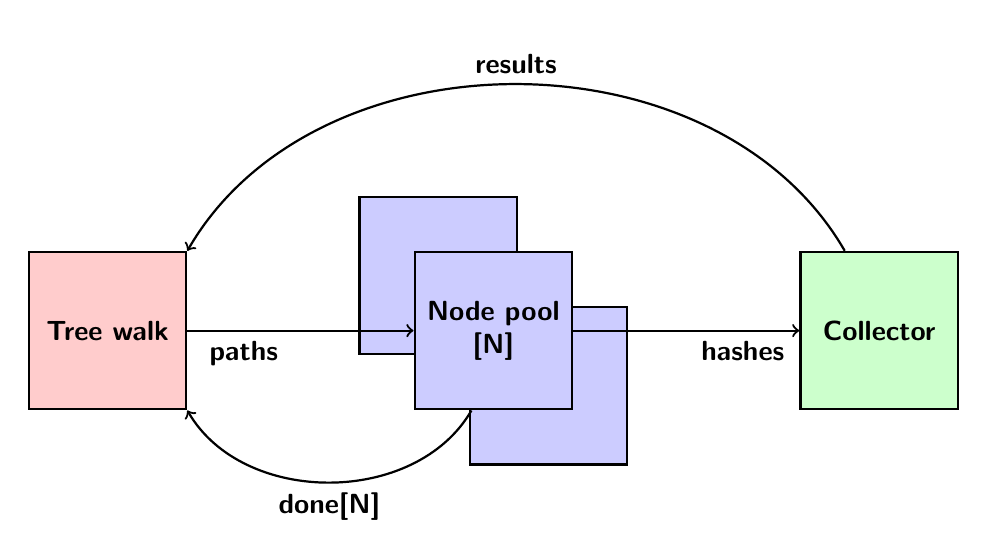
\begin{tikzpicture}[scale=0.7]            
            \tikzstyle{state}=[rectangle,minimum size=2cm,font=\sffamily\bfseries,draw]
            \tikzstyle{link}=[font=\sffamily\bfseries]

            \tikzstyle{every edge}=[thick,draw]

            \tikzstyle{M}=[state,thick,fill=green!20]    % main graph
            \tikzstyle{C}=[state,thick,fill=blue!20]     % clique
            \tikzstyle{A}=[state,thick,fill=red!20]      % key node

            \node[A] (0) at (-1, 0) {Tree walk};
            \node[C] (1) at ( 5, 1) {};
            \node[C] (1) at ( 7,-1) {};
            \node[C] (1) at ( 6, 0) [align=center]{Node pool\\ {[N]}};
            \node[M] (2) at (13, 0) {Collector};

            \tikzstyle{E}=[ultra thick,color=red]  % min cut

            \path[->] (0) edge node[link,below,near start] {paths}  (1);
            \path[->] (1) edge node[link,below,near end]   {hashes} (2);
            \path[->] (1) edge [bend left=60]  node[link,below] {done[N]} (0.south east);
            \path[->] (2) edge [bend right=60] node[link,above] {results} (0.north east);
        \end{tikzpicture}
    \end{center}
\end{frame}

\begin{frame}[fragile]
    \frametitle{How It Works: Collecting the Hashes}
\begin{golang}
func collectHashes(pairs <-chan pair, result chan<- results) {
	hashes := make(results)

	for p := range pairs {
		hashes[p.hash] = append(hashes[p.hash], p.path)
	}

	result <- hashes
}
\end{golang}
\end{frame}

\begin{frame}[fragile]
    \frametitle{How It Works: Replacing the Processor}
\begin{golang}
func processFiles(paths <-chan string, pairs chan<- pair,
                  done chan<- bool) {
	for path := range paths {
		pairs <- hashFile(path)
	}

	done <- true
}
\end{golang}
\end{frame}

\begin{frame}[fragile]
    \frametitle{How It Works: Replacing the Tree Walk}
\begin{golang}
workers := 2 * runtime.GOMAXPROCS(0)

paths := make(chan string)
pairs := make(chan pair)
done := make(chan bool, workers)  // buffered!
result := make(chan results)

for i := 0; i < workers; i++ {
	go processFiles(paths, pairs, done)
}

// we need another goroutine so we don't block here

go collectHashes(pairs, result)

. . .
\end{golang}
\end{frame}

\begin{frame}[fragile]
    \frametitle{How It Works: Replacing the Tree Walk}
\begin{golang}
err := filepath.Walk(dir, func(p string, fi os.FileInfo,
                               err error) error {
	// again, ignore the error passed in

	if fi.Mode().IsRegular() && fi.Size() > 0 {
		paths <- p
	}

	return nil
})

if err != nil {
    log.Fatal(err)
}

// we must close the paths channel so the workers stop
close(paths)
. . .
\end{golang}
\end{frame}

\begin{frame}[fragile]
    \frametitle{How It Works: Replacing the Tree Walk}
\begin{golang}
. . .

// wait for all the workers to be done

for i := 0; i < workers; i++ {
	<-done
}

// by closing pairs we signal that all the hashes
// have been collected; we have to do it here AFTER
// all the workers are done

close(pairs)

hashes := <-result

return hashes
\end{golang}
\end{frame}

\begin{frame}
    \frametitle{Evaluation \#1}
    \only<1-4>{56.11s in the version shown above \par}
    \vspace{\baselineskip}
    \only<2-4>{52.76s with a buffer to {\tt pairs} \par}
    \vspace{\baselineskip}
    \only<3-4>{51.36s with twice as many workers \par}
    \vspace{2\baselineskip}
    \only<4>{Buffering {\tt pairs} keeps the workers working \par}
    \vspace{\baselineskip}
\end{frame}

\section{Concurrent Approach \#2}
\begin{frame}
    \frametitle{Another Concurrent Approach}
    \only<1-5>{Add a goroutine for each directory in the tree \par}
    \vspace{\baselineskip}
    \only<2-5>{This improves the performance slightly, we're not waiting
               on paths to be identified \par}
    \vspace{2\baselineskip}
    \only<3-5>{51.14s in the basic version \par}
    \vspace{\baselineskip}
    \only<4-5>{50.03 adding buffers on channels to/from workers \par}
    \vspace{\baselineskip}
    \only<5>{48.75 with twice as many workers}
\end{frame}

\begin{frame}[fragile]
    \frametitle{How It Works: Parallel Tree Walk}
\begin{golang}
. . .

wg := new(sync.WaitGroup)

// multi-threaded walk of the directory tree; we need a
// waitGroup because we don't know how many to wait for

wg.Add(1)
err := walkDir(dir, paths, wg)

if err != nil {
	log.Fatal(err)
}

wg.Wait()
close(paths)

. . .
\end{golang}
\end{frame}

\begin{frame}[fragile]
    \frametitle{How It Works: Parallel Tree Walk}
\begin{golang}
func walkDir(dir string, paths chan<- string,
             wg *sync.WaitGroup) error {
	defer wg.Done()

	visit := func(p string, fi os.FileInfo, err error) error {
		// ignore the error passed in

        // ignore dir itself to avoid an infinite loop!
		if fi.Mode().IsDir() && p != dir {
			wg.Add(1)
			go walkDir(p, paths)
			return filepath.SkipDir
		}

        . . .
\end{golang}
\end{frame}

\begin{frame}[fragile]
    \frametitle{How It Works: Parallel Tree Walk}
\begin{golang}
        . . .

		if fi.Mode().IsRegular() && fi.Size() > 0 {
			paths <- p
		}

		return nil
	}

	return filepath.Walk(dir, visit)
}
\end{golang}
\end{frame}

\section{Concurrent Approach \#3}
\begin{frame}
    \frametitle{The Final Concurrent Approach}
    \only<1-5>{Use a goroutine for every directory and file hash \par}
    \vspace{\baselineskip}
    \only<2-5>{Without some controls, we'll run out of threads! \par}
    \vspace{2\baselineskip}
    \only<3-5>{We'll limit the number of {\bf active} goroutines instead \par}
    \vspace{\baselineskip}
    \only<4-5>{46.93s using 32 workers was the best time \par}
    \vspace{\baselineskip}
    \only<5>{Adding more workers actually makes the time grow longer }
\end{frame}

\begin{frame}
    \frametitle{Channels as Counting Semaphores}
    \only<1-5>{A goroutine can't proceed without sending on the channel \par}
    \vspace{\baselineskip}
    \only<2-5>{It must wait for another goroutine to receive \par}
    \vspace{2\baselineskip}
    \only<3-5>{The buffer allows a certain number to get running \par}
    \vspace{\baselineskip}
    \only<4-5>{And then one can start for each one that quits \par}
    \vspace{\baselineskip}
    \only<5>{We don't care how many goroutines exist at one time}
\end{frame}

\begin{frame}[fragile]
    \frametitle{How It Works: Limiting Goroutines}
\begin{golang}
// we don't need a channel for paths or to signal done but
// we need a buffered channel to act as a counting semaphore

wg := new(sync.WaitGroup)
limits := make(chan bool, workers)
pairs := make(chan pair, workers)
result := make(chan results)

go collect(pairs, result)

. . .
\end{golang}
\end{frame}
\begin{frame}[fragile]
    \frametitle{How It Works: Limiting Goroutines}
\begin{golang}
. . .

wg.Add(1)
err := walkDir(dir, pairs, wg, limits)

if err != nil {
	log.Fatal(err)
}

wg.Wait()
close(pairs)

hashes := <-result

return hashes
\end{golang}
\end{frame}

\begin{frame}[fragile]
    \frametitle{How It Works: Modified Processing}
\begin{golang}
func processFile(path string, pairs chan<- pair,
                 wg *sync.WaitGroup, limits chan bool) {
    defer wg.Done()

	limits <- true

	defer func() {
		<-limits		
	}()

	pairs <- hashFile(path)
}
\end{golang}
\end{frame}

\begin{frame}[fragile]
    \frametitle{How It Works: Modified Tree Walk}
\begin{golang}
func walkDir(dir string, pairs chan<- pair, wg *sync.WaitGroup,
             limits chan bool) error {
	defer wg.Done()

	visit := func(p string, fi os.FileInfo, err error) error {
		// ignore the error passed in

		if fi.Mode().IsDir() && p != dir {
			wg.Add(1)
			go walkDir(p, pairs, wg, limits)
			return filepath.SkipDir
		}

		. . .
\end{golang}
\end{frame}

\begin{frame}[fragile]
    \frametitle{How It Works: Modified Tree Walk}
\begin{golang}
        . . .

		if fi.Mode().IsRegular() && fi.Size() > 0 {
			wg.Add(1)
			go processFile(p, pairs, wg, limits)
		}

		return nil
	}

	limits <- true

	defer func() {
		<-limits
	}()

	return filepath.Walk(dir, visit)
}
\end{golang}
\end{frame}
\end{document}